% !TeX spellcheck = en_GB

\section{Algorithms}\label{algorithms}
\noindent Analogue to the script: \\
grammar $G=(V,\Sigma , S, P)$.\\
$V$ is a finite set of variables. \\
$\Sigma$ is an alphabet. \\
$S$ is the starting symbol and $S\ \epsilon\ V$. \\
$P$ is a finite set of rules: $P\ \subseteq\ V \times\ (V \cup\ \Sigma)^{*}$. \\ 
LHSE and RHSE are sets that shouldn't be defined. It is possible to have context free grammars(cfgs) with other kind of combinations.\\
$LHSE$ is finite set of left hand side elements: $LHSE = V$.\\
$RHSE$ is finite set of right hand side elements: $RHSE = (V \cup\ \Sigma)^{*}$.\\
$G.P.RHSE$ allows access to $RHSE$.\\
Variables that are of type set begin with a upper case letter.\\
$p.rhse$ allows access to the one specific $rhse$ of the specific production $p$.\\
So $P$ is a finite set of rules: $P\ \subseteq\ LHSE \times\ RHSE$. \\
Multisets allow duplicate elements. Notation of a multiset is done via the index b: $multiset_b$\\
pyramid is a structure where one $cell_{i,j}$ holds a set  $Cell_{i,j} = \{v\ |\ v\ \epsilon\ V\}$. If initialised each $cell_{i,j}$ holds $Cell_{i,j} = \emptyset $, which is named $empty\ pyramid$. $cell_{i+1,j} = cellDown;$ $cell_{i,j} = cellUpperLeft;\ cell_{i+1,j+1} = cellUpperRight;  $ \\
RHSEs are terminals like "a, b, ..." and compound variables like "AB, AC, ...". \\
LHSEs are variables like "A, B, ...".\\


\begin{figure}[h]
	\centering
	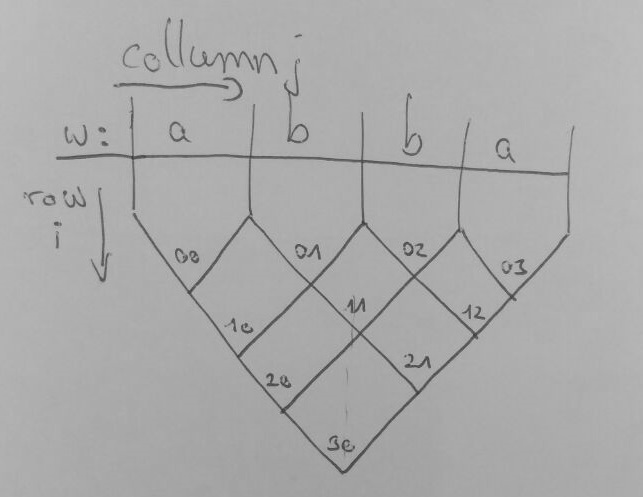
\includegraphics[width=0.7\textwidth]{abb/DataStructurePyramid}
\end{figure}

 \pagebreak 
 
\frame{
	\begin{algorithm}[H] %or another one check
		\caption{distributeRhseRandomly}
		\label{distributeRhseRandomly}
		\SetAlgoLined
		\KwIn{ $G,\ Rhse \subseteq\ RHSE,\ 0\leq minCount\leq maxCount\leq \mid G.V\mid$}
		\KwOut{$Grammar\ G\ with\ randomly\ distributed\ Rhse's.$}
		\ForEach {$rhse\ in\ Rhse$}{
			$addCount$ = $random(minCount, maxCount)$\;
			$VarsToAddTo = randomSubSet(addCount,\ LHSE)$\;
			
		
			\ForEach{var in VarsToAddTo}{
				$G.P = G.P\ \cup\ \{ "var\longrightarrow rhse" \} $\;	
			}
		}
		\Return $G$;
	\end{algorithm}
}
.\\
.\\
\frame{
	\begin{algorithm}[H] %or another one check
		\caption{GeneratorGrammarDiceRollMartens}
		\label{GeneratorGrammarDiceRollMartens}
		\SetAlgoLined
		\KwIn{ $word \in \Sigma^{*},\ V,\ \Sigma,\ S,\ P = \emptyset,\ minCount\Sigma,\ maxCount\Sigma,\ $ $ minCountVarComp,\ maxCountVarComp $ }
		\KwOut{$G$}
		
		$G=(V,\Sigma , S, P)$\;
		$G = distributeRhseRandomly(G,\ \Sigma,\ minCount\Sigma,\ maxCount\Sigma ) $\;
		$pyramid = CYK.calculatePyramid(G,\ word)$\;
		\ForEach{$cell_{i+1,j}\ in\ pyramid\ \wedge\ i>0$}{
			$VarComp = \{XY\ |\ X \in cellUpperLeft\ \wedge\ Y \in cellUpperRight \}$\;
			\ForEach{$vc\ in\ VarComp$}{
				\While{$cell_{wordLength+1,0} = \emptyset$}{
					$distributeRhseRandomly(G,\ vc,\ minCountVarComp,\ $ $maxCountVarComp ) $\;
					$pyramid = CYK.calculatePyramid(G,\ word)$\;	
				}
			}
		}
		\Return $G$\;
		\footnotetext{Line 3: Fills the i=0 row of the pyramid.\\
			\noindent Line 4: = foreach cellDown, but skipping the first row of the pyramid.
		}
	\end{algorithm}
}

 \pagebreak 
 
 
\frame{
 	\begin{algorithm}[H] %or another one check
 		\caption{checkRightCellCombination}
 		\label{checkRightCellCombination}
 		\SetAlgoLined
 		\KwIn{$ cellDown\subseteq V \,\ cellUpperLeft\subseteq V,\ cellUpperRight\subseteq V,\ G.P $ }
 		\KwOut{$varsThatForce\subseteq V$}
 		$isForced = false$\;
 		$VarsThatForce = \emptyset$\;
 		$VarComp = \{XY\ |\ X \in cellUpperLeft\ \wedge\ Y \in cellUpperRight \}$\;
 		\ForEach{$v\ in\ cellDown$}{
 			$VProd = \{p\ |\ p \in G.P\ \wedge\ p.lhse = v \}$\;
 			$VRhse = \{vRhse\ |\ vRhse \in VProd.RHSE \} $\;
 			\If{$VarComp \nsubseteq VRhse$}{
 				$isForced = true$\;
 				$VarsThatForce = VarsThatForce\ \cup\ v$\;
 			}			
 		}
 		\Return $VarsThatForce$\;
 	\end{algorithm}
}
\pagebreak


\frame{
 	\begin{algorithm}[H] %or another one check
 		\caption{checkRightCellCombinationForced}
 		\label{checkRightCellCombinationForced}
 		\SetAlgoLined
 		\KwIn{$ pyramid,\ G,\ minCountForced $ }
 		\KwOut{$G$}
 		$countForced = 0$\;
 		$isForced = true$\;
 		$varsThatForce = empty\ pyramid$\;
 		\ForEach{$cell_{i+1,j}\ in\ pyramid\ \wedge\ i>1 $}{
 			$varComp = \{XY\ |\ X\ \epsilon\ Cell_{i,j}\ \wedge\ Y\ \epsilon\ Cell_{i+1,j+1} \}$\;
 			
 			
 			
 			$ $\;
 		}
 		\Return $isForced,\ countForced,\ varsThatForce$\;
 		\footnotetext{Line 3: $i>1 \rightarrow$ the upper two rows aren't included, because they would produce trivial cases that fulfil the restriction always. 
 		}
 	\end{algorithm}
}
 
\pagebreak
 
\lstset{language=java}
\begin{lstlisting}[frame=htrbl, caption={distributeDiceRollRightHandSideElements}, 
label={lst:distributeDiceRollRightHandSideElements}]
Algorithm: distributeDiceRollRightHandSideElements
Input: grammar, setRhse, minCount, maxCount, listVars;
Output: grammar;

for(RightHandSideElement rhse : setRhse){
	// countWillBeAdded is between [minCount, maxCount]. 
	countWillBeAdded = diceRoll();
	while(listVars.size() > countWillBeAdded){
		Remove one variable of listVars via dice roll;
	}
	for(Variable varLeft : listVars){
		// An exception is thrown if the production 
		// already exists.
		grammar.addProduction "varLeft --> rhse";
	}
}
return grammar;
\end{lstlisting}


\lstset{}
\begin{lstlisting}[frame=htrbl, caption={distributeDiceRollRightHandSideElementsShort}, 
label={lst:distributeDiceRollRightHandSideElementsShort}]
Algorithm: distributeDiceRollRightHandSideElements
Input: grammar G, setRhse, minCount, maxCount, setGrammarVars;
Output: grammar;

foreach rhse in setRhse { 
	countWillBeAdded = dice roll a number within [minCount, maxCount];
	setVarsToAddRhse = {}dice roll countWillbeAdded to times vars from 	
		setGrammarVars that get the rhse added to;
	foreach var in setVarsToAddRhse {
		add production "var --> rhse" to grammar;
	}
}
return grammar;
\end{lstlisting}

\lstset{language=java}
\begin{lstlisting}[frame=htrbl, caption={CYK.calculateSetVAdvanced}, 
label={lst:CYK.calculateSetVAdvanced}]
Algorithm: CYK.calculateSetVAdvanced
Input: grammar, word;
Output: Set<VariableK>[][] cYKMatrix;

Set<VariableK>[][] cYKMatrix = new Set<VariableK>[wordSize][wordSize];
cYKMatrix = calculateCYKMatrix;
return cYKMatrix;
\end{lstlisting}

\pagebreak

\lstset{language=java}
\begin{lstlisting}[frame=htrbl,caption={GeneratorGrammarDiceRollTopDownMartens}, 
label={lst:GeneratorGrammarDiceRollTopDownMartens}]
Algorithm: GeneratorGrammarDiceRollTopDownMartens
Input: word, settings;
Output: grammar;
Note: Keep in mind that the setV matrix is a upper right matrix. But the
description of how the algorithm works is done, as if the setV pyramid 
points downwards (reflection on the diagonal + rotation to the left).
Regarding one cell, its upper left cell and its upper right cell 
are looked at. setV[i][j] = down cell. setV[i + 1][j] = upper right cell
setV[i][j - 1] = upper left cell. With wordSize = 5, the visited indexes 
are as following: [01->12->23->34; 02->13->24; 03->14; 04;]

Grammar grammar = new Grammar();
// Part1: Distribute the terminals.
grammar = distributeDiceRollRightHandSideElements(
	grammar, settingsTerminals, minCountTerminals, 
	maxCountTerminals, settingsListVariables);
// Part2: Distribute the compound variables.
Set<VariableKWrapper>[][] setVAdvanced;
// Fill the diagonal of the matrix with:
setVAdvanced = CYK.calculateSetVAdvanced( grammar, word );
for(Cell cellToBeVisited : setVAdvanced){
	setVariableCompound = calculate all the possible tupels of 
		({varLeft}, {varRight});
	for(VariableCompound varComp : setVariableCompound){
		// Because of dice rolling anyways and lots of grammars 
		// being generated, no varComp is added if the production
		// already exists.
		grammar = distributeDiceRollRightHandSideElements(
			grammar, varComp, minCountVarComp, 
			maxCountVarComp, settingsListVariables);
		setVAdvanced = CYK.calculateSetVAdvanced( grammar, word );
	}
}
return grammar;
// Forgot the while cell not empty do this from line 21 to line 33;
\end{lstlisting}

\pagebreak

\lstset{language=java}
\begin{lstlisting}[frame=htrbl,caption={GeneratorGrammarDiceRollOnly}, 
label={lst:GeneratorGrammarDiceRollOnly}]
Algorithm: GeneratorGrammarDiceRollOnly
Input: settings;
Output: grammar;
Note: A lot of productions are generated, that later on are not needed
for parsing the specific word.

Grammar grammar = new Grammar();
// Part1: Distribute the terminals.
grammar = distributeDiceRollRightHandSideElements(
	grammar, settingsTerminals, minCountTerminals, 
	maxCountTerminals, settingsListVariables);
// Part2: Distribute the compound variables.
Set<Variables> vars = settings.getVariables();
Set<VariablesCompound> setVarComp;
setVarComp = calculate all the possible tupels of ({vars}, {vars});
grammar = distributeDiceRollRightHandSideElements(
	grammar, settingsTerminals, minCountVariableCompound, 
	maxCountVariableCompound, setVarComp);
return grammar
\end{lstlisting}

\pagebreak

\lstset{language=java}
\begin{lstlisting}[frame=htrbl,caption={GeneratorGrammarDiceRollOnlyBias}, 
label={lst:GeneratorGrammarDiceRollOnlyBias}]
Algorithm: GeneratorGrammarDiceRollOnlyBias
Input: settings;
Output: grammar;
Note: A lot of productions are generated, that later on are not needed
for parsing the specific word.

Grammar grammar = new Grammar();
// Distribute the terminals.
grammar = distributeDiceRollRightHandSideElementsBias(
	grammar, settingsTerminals, settingsMinCountTerminals, 
	settingsMCountTerminals, settingsListVars, settingsFavouritism);

// Distribute the compound variables.
Set<VariablesCompound> setVarComp;
setVarComp = calculate all the possible tupels of ({vars}, {vars});
grammar = distributeDiceRollRightHandSideElementsBias(
	grammar, varComp, settingsMinCountVars,
	settingsMaxCountVars, settingsListVars, settingsFavouritism);
return grammar;
\end{lstlisting}

\pagebreak

\lstset{language=java}
\begin{lstlisting}[frame=htrbl,caption={distributeDiceRollRightHandSideElementsBias}, 
label={lst:distributeDiceRollRightHandSideElementsBias}]
Algorithm: distributeDiceRollRightHandSideElementsBias
Input: grammar, setRhse, minCount, maxCount, listVars, favouritismList;
Output: grammar;
Note: Because of dice rolling anyways and lots of grammars being 
generated, no rhse is added if the production already exists.

// Calculate the bloated varSet.
List<Variable> varsBloated;
for(Variables varTemp :  settings.getVariables()){
	tempFavour = randomly pick favouritism[i];
	varsBloated.add({tempFavour times varTemp});
	favouritism.remove(tempFavour);
}
// Because of dice rolling anyways and lot of grammars being generated, 
// just no rhse is added if the production already exists.
grammar = distributeDiceRollRightHandSideElements( grammar,
	varsBloated, minCount, maxCount, listVars );
return grammar;
\end{lstlisting}

\frame{
	\begin{algorithm}[H] %or another one check
		\caption{distributeDiceRollRightHandSideElementsBias}
		\label{distributeDiceRollRightHandSideElementsBias}
		\SetAlgoLined
		\KwIn{ $G,\ rhse \subseteq\ RHSE,\ 0\leq minCount\leq maxCount\leq\ \mid G.V\mid,\ favouritism = \{x\ |\ x\ \epsilon\ \mathrm{N}\ \wedge\ |favouritism| = |G.V| \}$}
		\KwOut{$G$}
		
		$favour = \{(v,\ f )\ |\ v\ \epsilon\ V \wedge\ f\ \epsilon\ favouritism\  \wedge\ tupel\ are\ created\ via\ dice\ roll \}$\;
		$varsBloated_b = \emptyset $\;
		\ForEach{fav in favour}{
			$varsBloated_b = varsBloated_b\ \biguplus\ \{ v^{f} \}$\;
		}
		\Return $distributeDiceRollRhse(
		G ,\ MISTAKEHEREvarsBloated_b,\ minCount,\ maxCount\ )$\;
		
		Still working on. One more Pprameter needed for distributeDiceRollRighthandSideElement. Parameter V that defines the variables the rhse are added to. OR make this algorithm independent.
		\footnotetext{Line 6: Note that $varsBloated_b$ is a multiset, but should actually be a set. Exceptions causing a duplicate production to
		the grammar are not relevant because G.P is a set. }
	\end{algorithm}
}

\pagebreak
\noindent Description of the checks here. \\
\noindent All test of the GrammarValidityChecker class are based on the simple setV matrix. \\

\noindent  isValid = isWordProducible \&\& isExamConstraints \&\& isGrammarRestrictions\\

\noindent  isWordProducible = CYK.algorithmAdvanced()\\

\noindent  isExamConstraints = isRightCellCombinationsForced \&\& isMaxSumOfProductionsCount \&\& isMaxSumOfVarsInPyramidCount \&\& countRightCellCombinationsForced \\

\noindent isGrammarRestrictions = isSizeOfWordCount \&\& isMaxNumberOfVarsPerCellCount \\

\lstset{language=java}
\begin{lstlisting}[frame=htrbl, caption={checksumOfProductions}, 
label={lst:checksumOfProductions}]
Algorithm: checksumOfProductions
Input: grammar, maxSumOfProduction;
Output: isSumOfProductions;

return grammar.getProductionsAsList().size() <= maxSumOfProductions; 
\end{lstlisting}

\pagebreak
\lstset{language=java}
\begin{lstlisting}[frame=htrbl, caption={checkMaxNumberOfVarsPerCell}, 
label={lst:checkMaxNumberOfVarsPerCell}]
Algorithm: checkMaxNumberOfVarsPerCell
Input: setVSimple, maxNumberOfVarsPerCell;
Output: isMaxNumberOfVarsPerCell;
Note: Checking for maxNumberOfVarsPerCell <= zero isn't allowed;

int tempMaxNumberOfVarsPerCell = 0;
int wordLength = tempSetV[0].length;
for ( int i = 0; i < wordLength; i++ ) {
	for ( int j = 0; j < wordLength; j++ ) {
		if ( tempSetV[i][j].size() > numberOfVarsPerCell ) {
			numberOfVarsPerCell = tempSetV[i][j].size();
		}
	}
}
return tempMaxNumberOfVarsPerCell <= maxNumberOfVarsPerCell;
\end{lstlisting}

\pagebreak

\lstset{language=java}
\begin{lstlisting}[frame=htrbl, caption={checkMaxSumOfVarsInPyramid}, 
label={lst:checkMaxSumOfVarsInPyramid}]
Algorithm: checkMaxSumOfVarsInPyramid
Input: setVSimple, maxSumOfVarsInPyramid;
Output: isMaxSumOfVarsInPyramid;

// put all vars of the matrix into one list and use its length.
List<Varaible> allVarsList = new ArrayList<>();
for ( int i = 0; i < setVSimple.length; i++ ) {
	for ( int j = 0; j < setVSimple.length; j++ ) {
		tempVars.addAll( setVSimple[i][j] );
	}
}
return allVarsList.size() <= maxSumOfVarsInPyramid; 
\end{lstlisting}

\pagebreak

\lstset{language=java}
\begin{lstlisting}[frame=htrbl, caption={rightCellCombinationsForced}, 
label={lst:rightCellCombinationsForced}]
Algorithm: rightCellCombinationsForced
Input: setVSimple, minCountForced, grammar;
Output: isForced, countForced, setVSimpleVarsThatForce;
Note: Keep in mind that the setV matrix is a upper right matrix. But the
description of how the algorithm works is done, as if the setV pyramid 
points downwards (reflection on the diagonal + rotation to the left).
Regarding one cell, its upper left cell and its upper right cell 
are looked at. setV[i][j] = down cell. setV[i + 1][j] = upper right cell
setV[i][j - 1] = upper left cell.

int countForced = 0;
Set<Variable>[][] setVMarkedVarsThatForce;
for(Cell cell : setVSimple){
	// Trivial cases that would fulfil the restrictions each time. 
	Ignore the upper two rows of the pyramid; 
	isRightCellCombinationForced = true;
	if(!upperLeftCell.isEmpty() && !upperRightCell.isEmpty()) {
		break;
	}
	setVariableCompound = calculate all the possible tupels of 
		({varLeft}, {varRight});
	for(Variable var : cellToBeVisited) {
		varDownProdList = grammar.getProdList(varDown);
		for(VariableCompound varComp : setVariableCompound) {
			for(Production prod : varDownProdList){
				if(prod.getRhse() == varComp) {
					isForced = false;
				}
			}
		}
		if(isRightCellCombinationForced) {
			rightCellCombinationsForced++;
			// Cell has index i and j.
			setVMarkedVarsThatForce[i][j].add(var)
		}
	}
}
boolean isForced = countForced >= minCountRightCellCombinationsForced;
return isForced, countForced, setVMarkedVarsThatForce;
\end{lstlisting}

\pagebreak

\lstset{language=java}
\begin{lstlisting}[frame=htrbl, caption={Util.removeUselessProductions}, 
label={lst:Util.removeUselessProductions}]
Algorithm: Util.removeUselessProductions
Input: grammar, setVSimple, word
Output: grammar
Note: Very similar to the calculateSetVAdvanced algorithm. Additionally
to storing the k, it is also saved, which production have been used. 
All productions that haven't been need are removed, from the grammar.

Set<Production> allProductions = grammar.getProductions();
Set<Production> onlyUsefulProductions;
onlyUsefulProductions = calculate useful productions with the input of
	grammar, setVSimple and word ;
grammar.remove(allProductions);
return grammar.add(onlyUsefulProductions);
\end{lstlisting}

\pagebreak